\section{Virtual Threads: La Base}

\begin{frame}
\frametitle{Virtual Threads: M:N Mapping}

\begin{columns}
\column{0.48\textwidth}
\begin{center}
\textbf{\small Platform Threads (1:1)}

\vspace{0.5em}
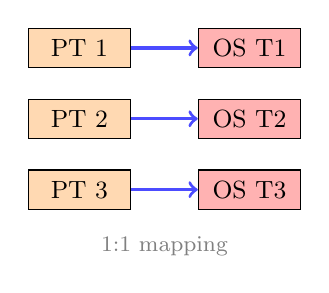
\begin{tikzpicture}[scale=0.9]
    % Platform threads on the left
    \node[draw, fill=orange!30, minimum width=1.3cm, minimum height=0.5cm, font=\small] (p1) at (-1.2,1.8) {PT 1};
    \node[draw, fill=orange!30, minimum width=1.3cm, minimum height=0.5cm, font=\small] (p2) at (-1.2,0.8) {PT 2};
    \node[draw, fill=orange!30, minimum width=1.3cm, minimum height=0.5cm, font=\small] (p3) at (-1.2,-0.2) {PT 3};

    % OS threads on the right - moved further right
    \node[draw, fill=red!30, minimum width=1.3cm, minimum height=0.5cm, font=\small] (o1) at (1.2,1.8) {OS T1};
    \node[draw, fill=red!30, minimum width=1.3cm, minimum height=0.5cm, font=\small] (o2) at (1.2,0.8) {OS T2};
    \node[draw, fill=red!30, minimum width=1.3cm, minimum height=0.5cm, font=\small] (o3) at (1.2,-0.2) {OS T3};

    % Clean 1:1 arrows - now longer
    \draw[->, very thick, blue!70] (p1) -- (o1);
    \draw[->, very thick, blue!70] (p2) -- (o2);
    \draw[->, very thick, blue!70] (p3) -- (o3);

    \node[gray, font=\footnotesize] at (0,-1) {1:1 mapping};
\end{tikzpicture}
\end{center}

\column{0.48\textwidth}
\begin{center}
\textbf{\small Virtual Threads (M:N)}

\vspace{0.5em}
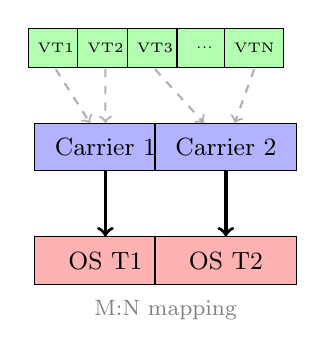
\begin{tikzpicture}[scale=0.9]
    % Virtual threads layer
    \node[draw, fill=green!30, minimum width=0.7cm, minimum height=0.5cm, font=\tiny] at (-1.2,2.2) {VT1};
    \node[draw, fill=green!30, minimum width=0.7cm, minimum height=0.5cm, font=\tiny] at (-0.5,2.2) {VT2};
    \node[draw, fill=green!30, minimum width=0.7cm, minimum height=0.5cm, font=\tiny] at (0.2,2.2) {VT3};
    \node[draw, fill=green!30, minimum width=0.7cm, minimum height=0.5cm, font=\tiny] at (0.9,2.2) {...};
    \node[draw, fill=green!30, minimum width=0.7cm, minimum height=0.5cm, font=\tiny] at (1.6,2.2) {VTN};

    % Carrier threads
    \node[draw, fill=blue!30, minimum width=1.8cm, minimum height=0.6cm, font=\small] (c1) at (-0.5,0.8) {Carrier 1};
    \node[draw, fill=blue!30, minimum width=1.8cm, minimum height=0.6cm, font=\small] (c2) at (1.2,0.8) {Carrier 2};

    % OS threads
    \node[draw, fill=red!30, minimum width=1.8cm, minimum height=0.6cm, font=\small] (os1) at (-0.5,-0.8) {OS T1};
    \node[draw, fill=red!30, minimum width=1.8cm, minimum height=0.6cm, font=\small] (os2) at (1.2,-0.8) {OS T2};

    % Connections
    \draw[->, thick, dashed, gray!60] (-1.2,1.9) -- (c1);
    \draw[->, thick, dashed, gray!60] (-0.5,1.9) -- (c1);
    \draw[->, thick, dashed, gray!60] (0.2,1.9) -- (c2);
    \draw[->, thick, dashed, gray!60] (1.6,1.9) -- (c2);

    \draw[->, very thick] (c1) -- (os1);
    \draw[->, very thick] (c2) -- (os2);

    \node[gray, font=\footnotesize] at (0.35,-1.5) {M:N mapping};
\end{tikzpicture}
\end{center}
\end{columns}

\vspace{0.5em}
\begin{block}{Ventajas Clave}
\begin{itemize}
\item Millones de Virtual Threads con pocos OS Threads
\item Muy bajo costo de creación (~1KB vs ~2MB)
\item Scheduling inteligente (park/unpark automático)
\end{itemize}
\end{block}
\end{frame}

\begin{frame}
\frametitle{Virtual Threads: La Base de Structured Concurrency}

\begin{exampleblock}{¿Por qué Virtual Threads habilitan Structured Concurrency?}
\begin{itemize}
\item \textbf{Bajo Costo:} Crear miles de tareas ya no es problema
\item \textbf{Blocking is OK:} Puedes escribir código bloqueante simple
\item \textbf{Natural Structure:} fork/join patterns son eficientes
\item \textbf{No más thread pools:} Un thread por task, administración automática
\end{itemize}
\end{exampleblock}

\vspace{1em}
\begin{block}{Comparación de Costos}
\begin{center}
\begin{tabular}{|l|c|c|}
\hline
\textbf{Recurso} & \textbf{Platform Thread} & \textbf{Virtual Thread} \\
\hline
Memoria (stack) & ~2 MB & ~1 KB \\
Tiempo creación & ~1 ms & ~1 \textmu{}s \\
Context switch & ~10 \textmu{}s & ~1 \textmu{}s \\
Máximo práctico & ~miles & ~millones \\
\hline
\end{tabular}
\end{center}
\end{block}

\vspace{0.5em}
\begin{alertblock}{Resultado}
Virtual Threads hacen viable el modelo fork/join masivo de Structured Concurrency
\end{alertblock}
\end{frame}

\begin{frame}
\frametitle{El Problema: Procesamiento de Transacción Financiera}
\begin{center}
\Large{Flujo ficticio de Validación y Débito de una transacción financiera}
\end{center}

\vspace{1em}
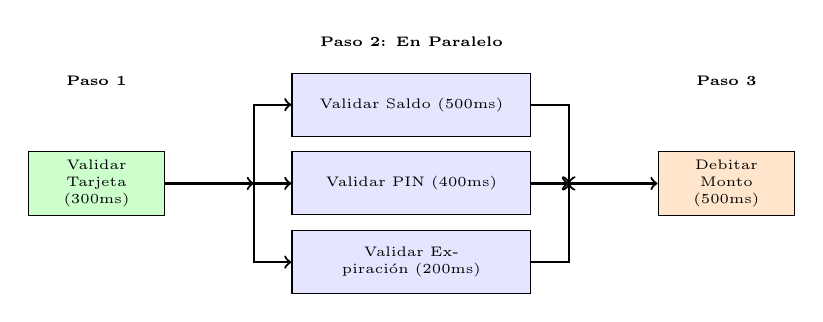
\begin{tikzpicture}[
    node/.style={draw, rectangle, text width=1.5cm, align=center, font=\tiny, minimum height=0.8cm},
    parallel/.style={draw, rectangle, text width=2.8cm, align=center, font=\tiny, fill=blue!10, minimum height=0.8cm},
    arrow/.style={->, thick}
]

% Nodes positioned manually for precise alignment
\node (card) [node, fill=green!20] at (0,0) {Validar \\ Tarjeta \\ (300ms)};

% Parallel validations - perfectly aligned vertically
\node (balance) [parallel] at (4,1) {Validar Saldo (500ms)};
\node (pin) [parallel] at (4,0) {Validar PIN (400ms)};
\node (expiry) [parallel] at (4,-1) {Validar Expiración (200ms)};

\node (debit) [node, fill=orange!20] at (8,0) {Debitar \\ Monto \\ (500ms)};

% Coordination points for line division and convergence
\coordinate (split) at (2,0);
\coordinate (join) at (6,0);

% Arrows with structured lines
% From card to split point
\draw [arrow] (card.east) -- (split);

% From split point to parallel validations (vertical then horizontal)
\draw [arrow] (split) -- (2,1) -- (balance.west);
\draw [arrow] (split) -- (pin.west);
\draw [arrow] (split) -- (2,-1) -- (expiry.west);

% From parallel validations to join point (horizontal then vertical)
\draw [arrow] (balance.east) -- (6,1) -- (join);
\draw [arrow] (pin.east) -- (join);
\draw [arrow] (expiry.east) -- (6,-1) -- (join);

% From join point to debit
\draw [arrow] (join) -- (debit.west);

% Labels
\node [above of=card, yshift=0.3cm, font=\tiny]{\textbf{Paso 1}};
\node [above of=pin, yshift=0.8cm, font=\tiny] {\textbf{Paso 2: En Paralelo}};
\node [above of=debit, yshift=0.3cm, font=\tiny]{\textbf{Paso 3}};

\end{tikzpicture}

\vspace{0.5em}
\begin{alertblock}{Flujo Optimizado}
\textbf{1.} Validar tarjeta primero (paso previo para obtener el resto de la información)\\
\textbf{2.} Validaciones paralelas si tarjeta OK\\
\textbf{3.} Debitar solo si todas las validaciones pasan
\end{alertblock}
\end{frame}

